% Copy figures/winning_color_leaf.png into the paper figures/ folder.
% Distinct from K-means clustering (Fig.~\ref{fig:clustering}): this colors
% anchors by the color router, not by a partition of f_v.

\section{Winning color-leaf assignment}
\label{app:winning-leaf}

Anchor-feature clustering (Fig.~\ref{fig:clustering}) is Scaffold-GS's
protocol~\cite{lu2024scaffold}: K-means with \(K{=}3\) on the stored
feature \(f_v\in\mathbb{R}^{32}\).
That experiment asks whether \(f_v\) still separates floor from furniture.
It does \emph{not} say which expert paints the Gaussian.

The decoder used at render time is the color router.
For each visible anchor \(i\) we take the color-head gate on
\(z_i=f_i\) (no view direction, no GNN) and assign
\begin{equation}
  \ell^\star_i
  =
  \arg\max_{\ell}
  \pi_i(\ell).
\end{equation}
Figure~\ref{fig:winning-leaf} colors the same 30k anchors by \(\ell^\star_i\).
The legend on each panel is the leaf index \(L_\ell\) and its mass
(fraction of in-room anchors).
Scaffold-GS is omitted: a shared MLP has one expert, so every anchor would
be the same color.

On Deep Blending \texttt{playroom}, flat MoE uses all 8 color experts,
with mass peaked on \(L_3\) (\(26\%\)) then \(L_0\) and \(L_6\)
(\(\approx 18\%\) each); \(L_1\) is unused (\(<0.1\%\)).
Tree MoE occupies 10 of 11 color leaves.
The split parent is empty, and mass is flatter
(\(L_3,L_0,L_9,L_2\) each hold \(13\)--\(15\%\)).
On Mip-NeRF~360 \texttt{kitchen} the same pattern holds:
flat MoE spreads over 8 experts (\(L_6\) \(19\%\), \(L_1\) and \(L_0\)
\(\approx 17\%\)); the tree uses 10 leaves, leaves the grown-out parent
empty, and does not collapse onto one specialist.

The 3D map is spatially structured---floor versus furniture on
\texttt{playroom}, table versus clutter on \texttt{kitchen}---but it is an
8- or 10-way assignment, not a \(K{=}3\) partition, so neighboring anchors
can take different leaves.
That speckle is expected: Top-2 routing is local in \(f_v\), not a hard
spatial Voronoi.
\(L_\ell\) in flat MoE is expert \(\ell\) of 8;
\(L_\ell\) in Tree MoE is color-leaf \(\ell\) of the grown tree.
After a split those indices are not the same physical expert.

\begin{figure*}[t]
  \centering
  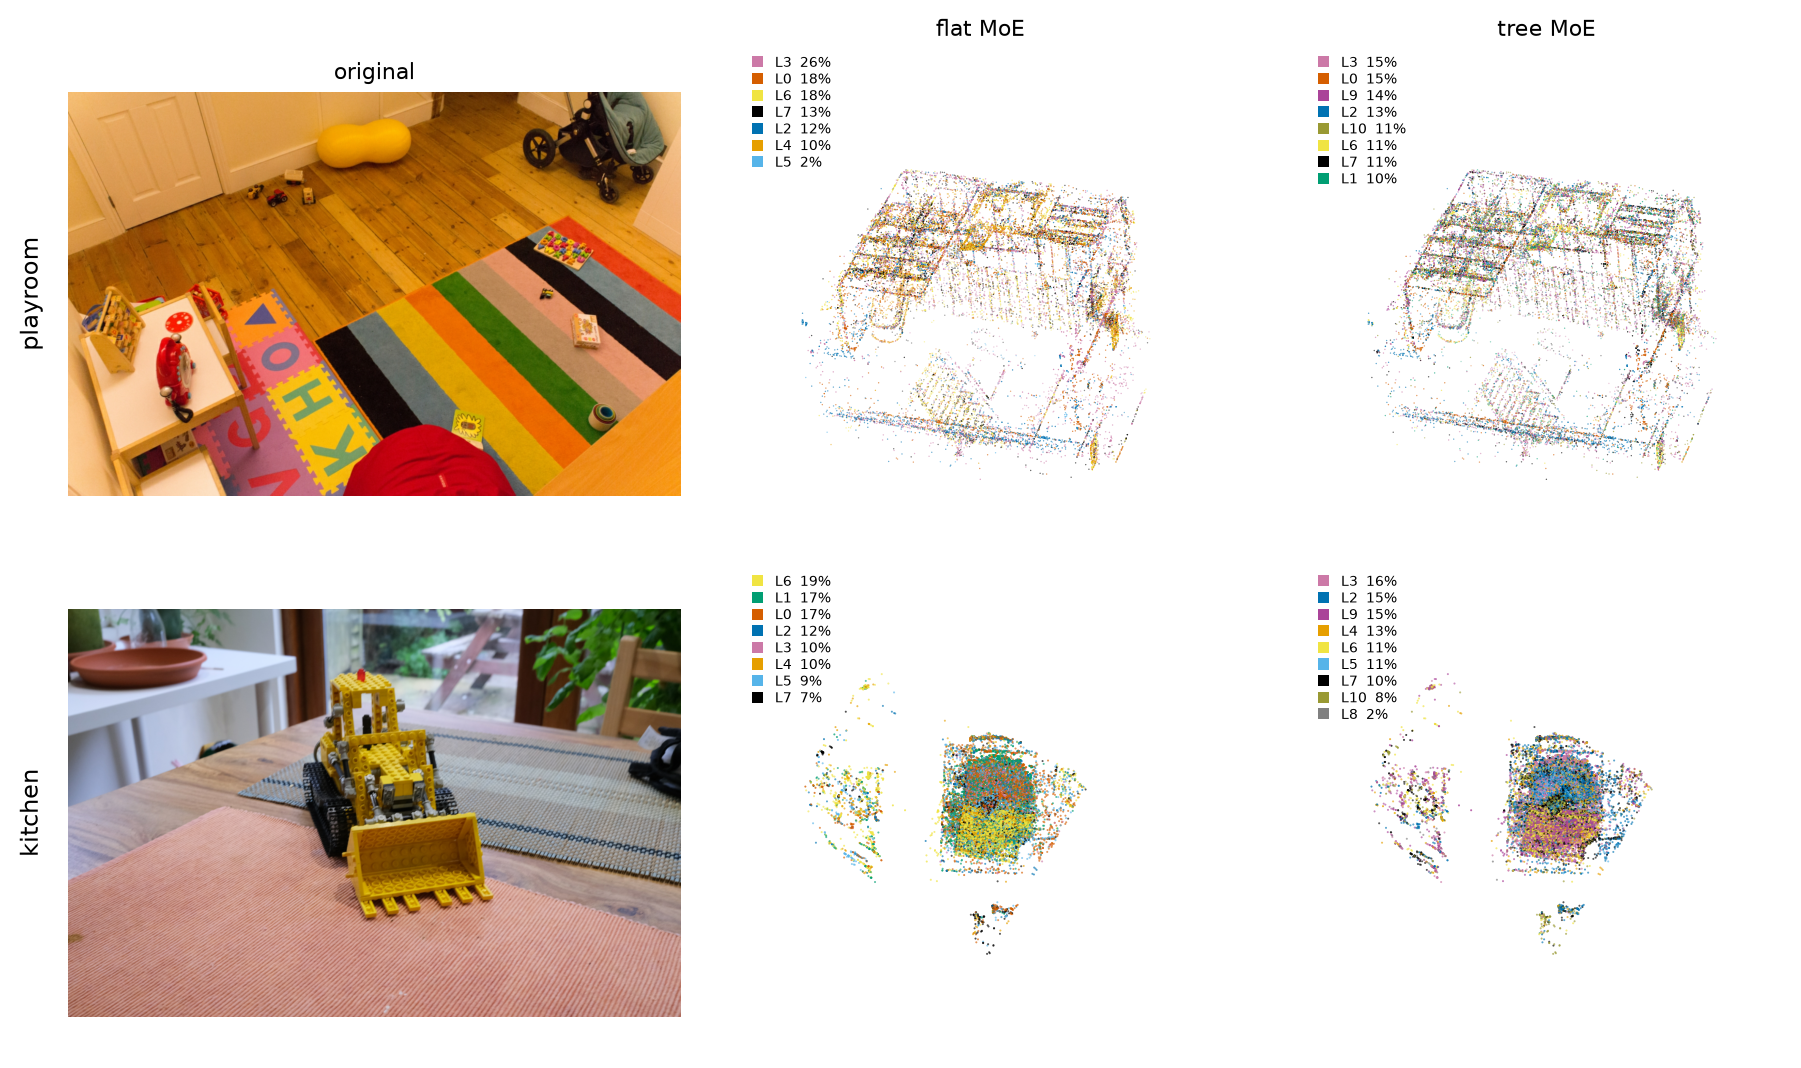
\includegraphics[width=\linewidth]{figures/winning_color_leaf.png}
  \caption{\textbf{Anchors colored by the winning color leaf.}
  Each point is an anchor; color is
  \(\ell^\star=\arg\max_\ell\pi(\ell)\) of the color router on \(z{=}f_v\).
  Rows: Deep Blending \texttt{playroom}, Mip-NeRF~360 \texttt{kitchen}.
  Columns: original image, flat MoE (8 leaves), Tree MoE (10 used leaves).
  Legend: leaf index and mass share.
  This is \emph{not} K-means on \(f_v\) (cf.\ Fig.~\ref{fig:clustering}).}
  \label{fig:winning-leaf}
\end{figure*}
